\usetikzlibrary{positioning,arrows.meta,fit,shadows,backgrounds}
\begin{figure}[h]
  \centering
  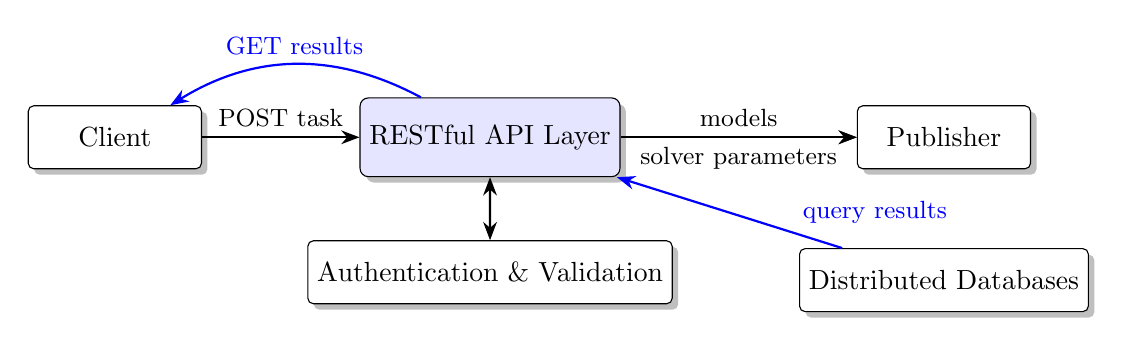
\begin{tikzpicture}[
      scale=0.8,
      >=Stealth,
      box/.style={draw,rectangle,rounded corners=2pt,minimum width=2.2cm,
                  minimum height=0.8cm,align=center,fill=white,drop shadow},
      apibox/.style={draw,rectangle,rounded corners=3pt,minimum width=2.8cm,
                  minimum height=1cm,align=center,fill=blue!10,drop shadow},
      msg/.style={->, thick},
      label/.style={font=\small,draw=none}
    ]
    
    % Client
    \node[box] (client) {Client};
    
    % REST API Layer with its components
    \node[apibox, right=2cm of client] (api) {RESTful API Layer};
    \node[box, below=0.8cm of api] (auth) {Authentication \& Validation};
    
    % Publisher
    \node[box, right=3cm of api] (publisher) {Publisher};
    
    % Database
    \node[box, below=1cm of publisher] (db) {Distributed Databases};
    
    % Fit node for Backend System
    \node[fit=(api)(auth)(publisher)(db),
          draw, inner sep=0.3cm, dashed, 
          label={[yshift=0.3cm]\textbf{Backend System}}] (platform) {};
    
    % Draw connections
    \draw[msg] (client) -- node[above,label]{POST task} (api);
    \draw[msg] (api) -- node[above,label]{models} (publisher);
    \draw[msg] (api) -- node[below,label]{solver parameters} (publisher);

    % Two-way arrow between API and Auth
    \draw[<->, thick] (api) -- (auth);
    
    % Status monitoring path
    \draw[msg, blue] (api) to[bend right=30] node[above,label] {GET results} (client);
    
    % Database connections
    \draw[msg, blue] (db) -- node[right,xshift=0.8cm,label]{query results} (api);
    
  \end{tikzpicture}
  \caption{Simplified RESTful API architecture for PRA task management.}
  \label{fig:rest-api-architecture}
\end{figure}